\documentclass[11pt]{article}

\usepackage[english]{babel}
\usepackage{url}
\usepackage{graphicx,style_in}
\usepackage{float} 
\usepackage{subfig}
\usepackage{mathtools}

\pagestyle{fancy} 
\fancyhead{} 
\fancyfoot{} 
\linespread{0.9}

\usepackage{amsmath}

\makeatletter

\fancyhead[RO]{\small The International Summer Conference on Theoretical Physics 2023\\ {Abrikosov Center for Theoretical Physics}}

\title{Simulation of Two-Phase Flow in Porous Media using a Two-Dimensional Network Model}

\author{K. Shabbir$^1$}
\author{O. Izvekov$^2$}
\author{A. Konyukhov$^3$}

\affil{$^{1, 2, 3}$Moscow Institue of Physics and Technology}
\email{$^1$kafiulshabbir@phystech.edu, $^2$izvekov\_o@inbox.ru, $^{3}$konyukhov\_av@mail.ru}

\begin{document}
	\maketitle
	
	\vskip -1.5em

	\begin{abstract}
	
		Various algorithms and methods used to simulate two-phase flow in porous media has many
		practical applications in oil recovery, hydrology, electricity production where pressurized water is passed through heated pipes and is transformed into steam, etc. The algorithm presented here is used to find the saturation of a phase with respect to time and model imbibition.
		
		\keywords{Two-phase flow, porous body, imhibition}
		
	\end{abstract}
	
	\section*{Introduction}
		Figure \ref{fig:example-porous-body} is an example of two-phase flow in porous body. The wetting fluid, in this case - water displaces the non wetting fluid - air. The aim is to plot concentration of one of the phases with respect to time for a given region of the porous body, similar to \cite{bib1}.
		
		
		\begin{figure}[H]
			\centering
			\subfloat[Porous body]{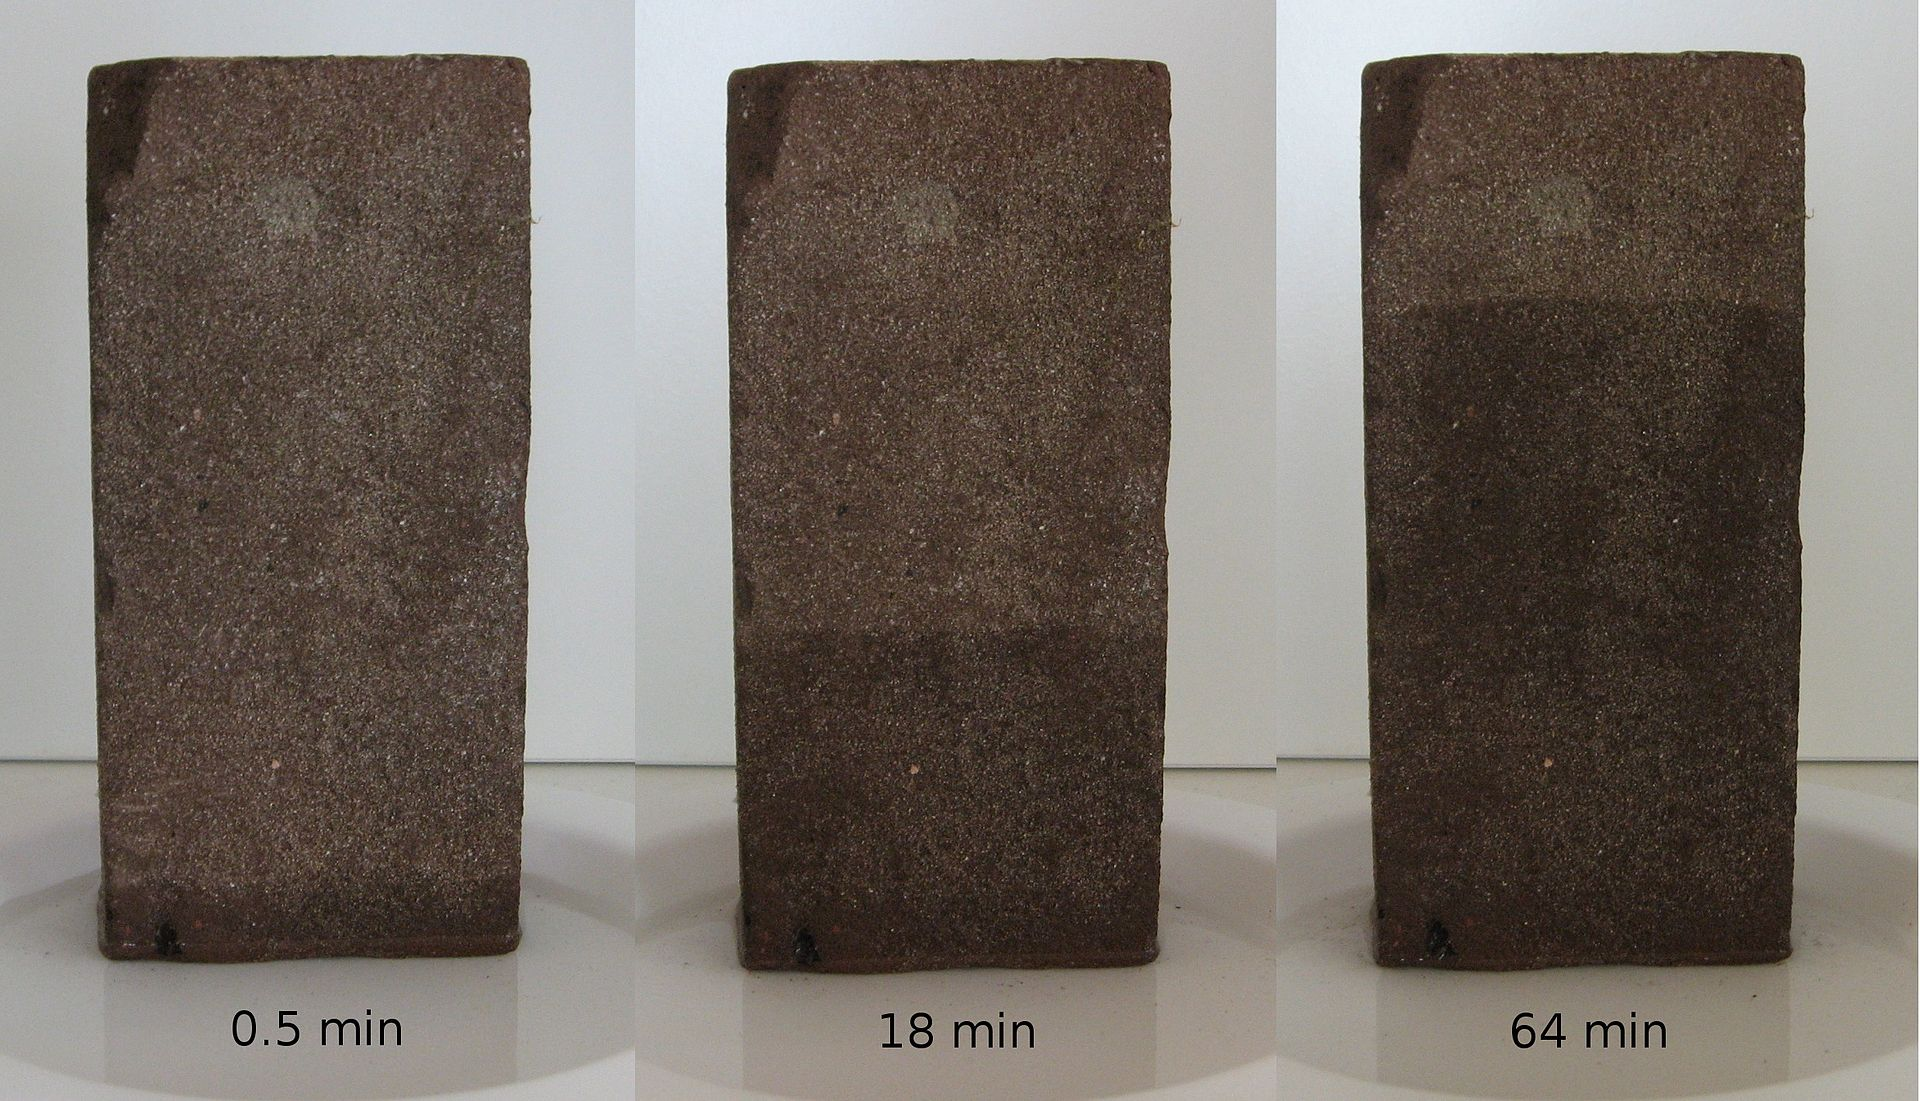
\includegraphics[height=4.2cm]{example-porous-body}\label{fig:example-porous-body}}
			\subfloat[Model]{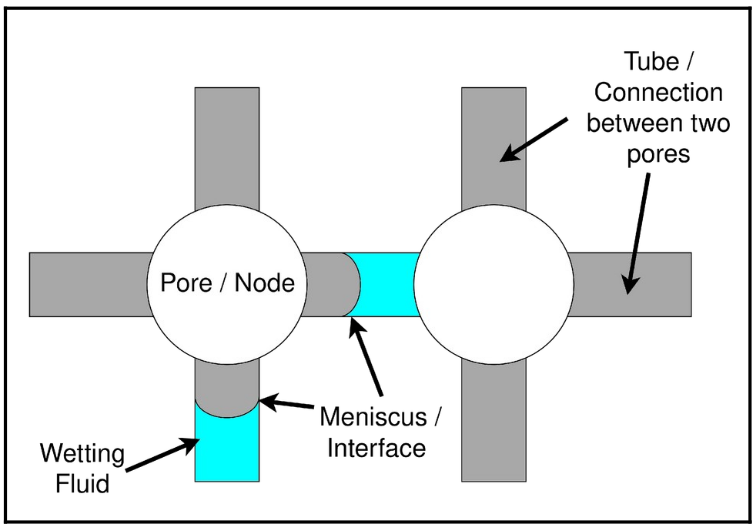
\includegraphics[height=4.2cm]{modeling-basic}\label{fig:modeling-basic}}
			\caption{Example of two-phase flow in porous body and a simplified manner of modeling the process}
		\end{figure}
	
	\section*{Model}		
		The flow rate when a tube contain meniscus after necessary derivation is given by a modified Poiseuille's equation:
		\begin{equation} \label{eq:flow-rate-main}
			Q_{ij} = \frac{\pi R_{ij}^4}{8M_{ij}l} \left(\Delta P_{ij} + \frac{2s_{ij}\sigma}{R_{ij}} \right)
		\end{equation}
		
		Here $M_{ij}$ is:
		\begin{equation}
			{M}_{ij} = \sum_{k} {\mu}_{ijk} \frac{l_{ijk}}{l}
		\end{equation}
		
		And 
		$s_{ij} = \{-1, 0, +1\}$ depending on the orientation and number of meniscus.
		
		For every node due to conservation of volume:
		\begin{equation}
			\sum_j Q_{ij} = 0
		\end{equation}
		
		This produces $n$ linear equations for a model with $n$ nodes. The pressures at each node are the variables. Gaussian-elimination is used to solve the linear equations. This is the most computationally expensive task and defines for how many nodes, the simulation can be performed in a given time. Various methods of optimizations have been presented in \cite{bib4}.
	
	The calculated pressures at each node is used to determine the flow rates according to equation \ref{eq:flow-rate-main}. Then the time step is decided and each meniscus in the tubes is displaced according to $d_{ij} = v_{ij} \Delta t_{ij}$. The novelty of our algorithm is the distribution of the phases when more than one phase enters a node. The wetting fluid is distributed first in ascending order of the radius of the tubes. After this if there are more than two meniscus in a tube, the phases are combined such that the center of mass of the phases remain the same. This algorithm can be extended to the case of a 3-D model, such as in \cite{bib2}.
		
	\section*{Results}
		For modeling only the saturation of a phase in a given region \cite{bib5} when there is an external pressure difference, does not produce oscillations unlike modeling imhibition where the boundaries are closed and the volume of each phase in the system remains the same. Here the fluid does not reach an equilibrium position in a finite amount of time. However the small oscillations dampens over time, as in figure \ref{fig:sat-vs-time}. Another significant advantage of this method is that the shape of the tubes are considered to be cylindrical unlike hour glass shape in \cite{bib3} and and flow is determined by solving a set of linear equations. Computation requires a few hours for 30x30 matrix of tubes on a personal computer.
		\begin{figure}[H]
			\centering
			\subfloat[Initial]{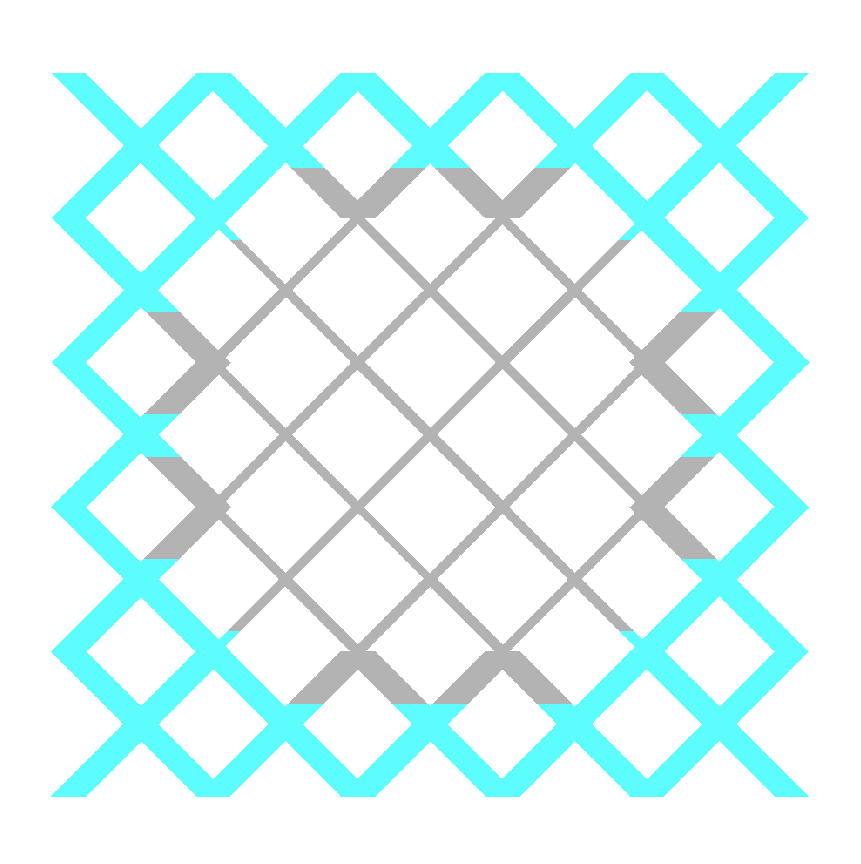
\includegraphics[height=4cm]{res-pic1}}
			\subfloat[Invasion]{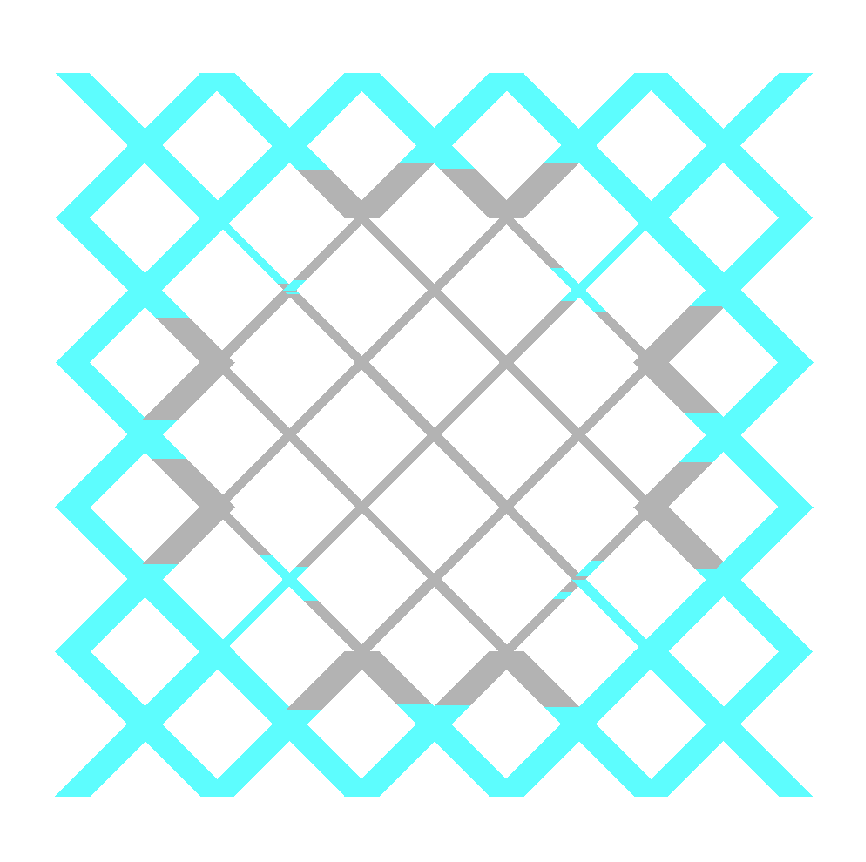
\includegraphics[height=4cm]{res-pic2}}
			\subfloat[Final]{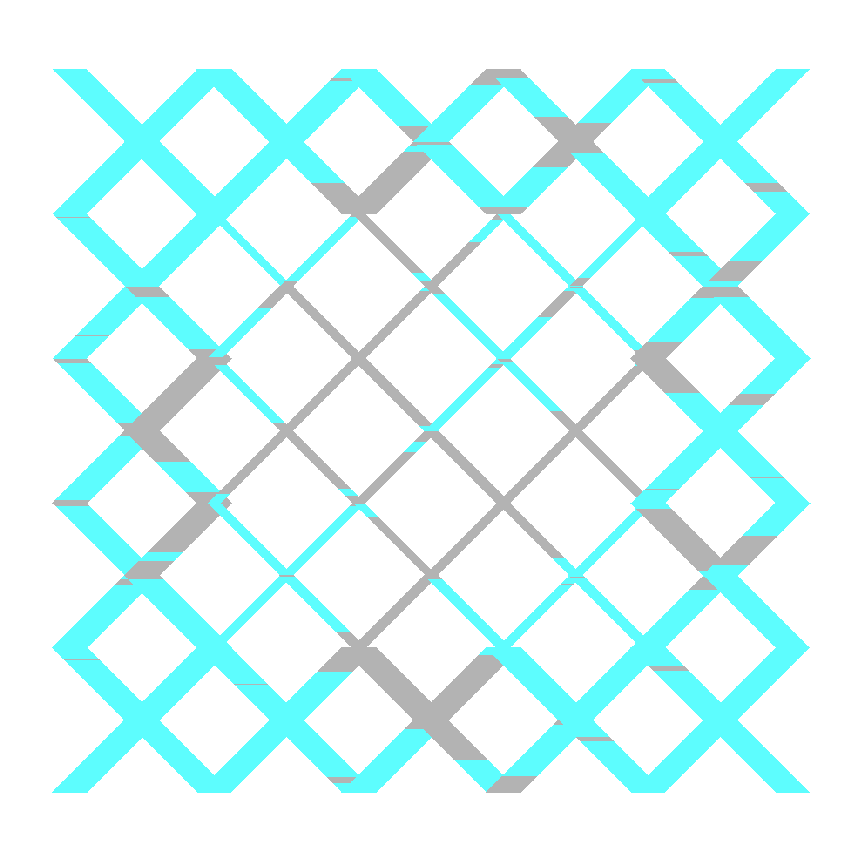
\includegraphics[height=4cm]{res-pic3}}
			\caption{Showing how a wetting fluid enters the region with thinner radius}
		\end{figure}
		\begin{figure}[H]
			\centering
			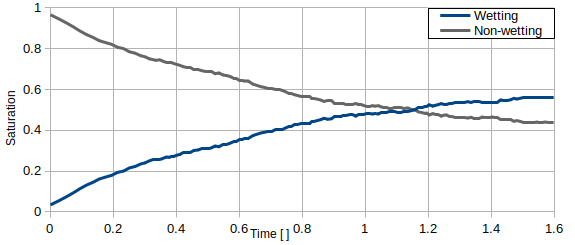
\includegraphics[width=0.5\textwidth]{plot-sat-vs-time}
			\caption{Volumetric saturation of the two-phases in the region of thinner radius with respect to dimensionless time}
			\label{fig:sat-vs-time}
		\end{figure}
	This work was supported by grant RNF 23-21-00175.
	\begin{thebibliography}{}
		\bibitem{bib1}  %% citation code
			 Fatt I. The network model of porous media 3, dynamic properties of networks with tube radius distribution Petroleum Trans. AIME 1956. V. 207. P. 164
		
		\bibitem{bib4}
			Raoof A., Hassanizadeh S. A new method for generating pore-network models of porous media // Transp. Porous Med. 2010. V. 81. P. 391
			 
		\bibitem{bib2}
			S. Sinha et al. Effective rheology of two-phase flow in three-dimensional porous media: experiment and simulation // Transp. Porous Med. 2017. V. 119. P. 77
			
		\bibitem{bib5}
			K. Shabbir, Sim of Two-Phase flow network model, 65 All Russia Scientific Conference MIPT, Aerospace Section, P. 196, https://mipt.ru/upload/medialibrary/002/aerokosmicheskie-tekhnologii.pdf
			
		\bibitem{bib3}
			Aker E., Måløy K et al. A two-dimensional network simulator for two-phase flow in porous media // Transp. Porous Med. 1998 V. 32 P. 163
	
	\end{thebibliography}

\end{document}
